\subsection{Definition}
The Lagrangian relaxation is a procedure that find a \textbf{lower
bounds}. This
lower bounds will allow to have better performances on the branch and
bounds of the problem starting with an initially good lower-bounds.

\begin{enumerate}
    \item We first relax the problem with the Lagrangian relaxation 
    \item We optimize the $\lambda$ with a sub-gradient algorithm 
    \item We get the optimal $\lambda$ and thus the optimal solution of
        the relaxed problem which is a good lower bounds.
\end{enumerate}

\subsection{Constrained Shortest Path Problem}
In order to represents the concepts discussed in this section, we will
need an example. Lets take the Constrained Shortest Path problem.

\begin{tabular}{m{8cm}m{6cm}}
    \begin{eqnarray*}
        \textrm{minimize } & \sum_{(i,j) \in A} c_{ij} \quad x_{ij} \\
        \textrm{subject to } & \textrm{flow conservation}\\
                            & \sum_{(i,j) \in A } \quad t_{ij} x_{ij} \leq T \\
                             & \forall (i, j) \in A, \quad x_{ij} \in \{0, 1\}
        \end{eqnarray*}

        \begin{itemize}
            \item A example can be to minimize distance with
                \textbf{time constraint} (NP-Hard problem).
        \end{itemize}
& 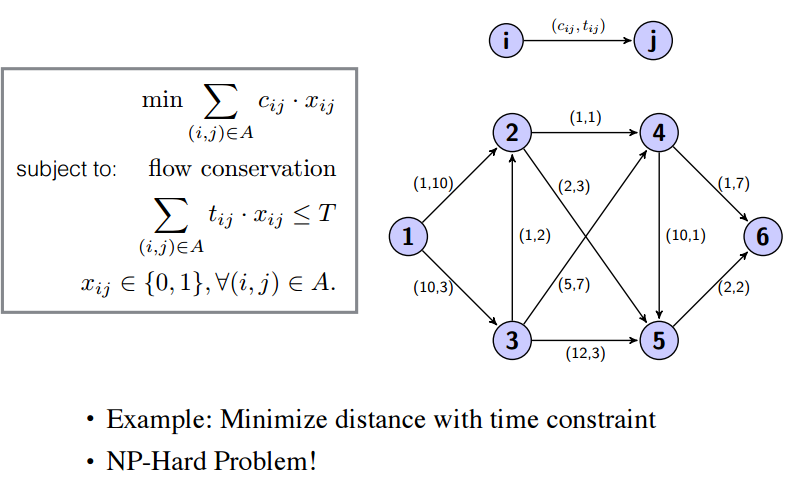
\includegraphics[width=7cm]{lagrangeexample.png}
\end{tabular}


\subsection{Relaxation}

If we remove the resource constraint, the problem is pretty easy. It is
a simple shortest path problem that can be easily resolved with
Dijkstra. What the Lagrangian relaxation does is \textbf{removing the
constraint} and \textbf{adding a new part} in our minimization part.

\begin{eqnarray*}
    L(\lambda) &=& min \sum_{(i,j)\in A} c_{ij} x_{ij} + 
    \textcolor{red}{\lambda \bigg(\sum_{(i,j)\in A} t_{ij} x_{ij} - T
    \bigg)} \\
    %&=& min \sum_{(i,j)\in A} \Big(c_{ij} + \lambda t_{ij}\Big) x_{ij} - \lambda T\\
\end{eqnarray*}

$\Rightarrow$ We now have a simple shortest path problem 
where edges has a weight which is a
mixed value of time and distance for a given value of $\lambda$. 

\begin{itemize}
    \item Using this minimization with different $\lambda$ will return
        different solutions. 

    \item Some of them won't be feasibly and will violate the time
        constraint. If you are lucky one of the solution will be the
        optimal one. (hint: try $\lambda = 2$)
\end{itemize}

\subsection{Lagrangian dual}
Now our objective will be to find the best $\lambda$ in order to have
the best feasible solution (the best we can have with Lagrangian, not
necessarily the best of the actual problem, this algorithm is only used
to have a lower bound). We have our Lagrangian dual: 
$$L* = max_{\lambda} \Bigg( min \sum_{(i,j)\in A} (c_{ij} + x_{ij}) +
\lambda \big(\sum_{(i,j)\in A} (t_{ij} x_{ij}) - T\big) \Bigg)$$

\paragraph{Idea}
The idea, according to Nicolas Houtain, is that 
\begin{itemize} 
    \item we know that as the minimum value are convex and that the max
        value on these minimum value are the point where we pass from 
        unfeasible path to feasible path

    \item So, the max value is the feasible path with minimum value. We
        want to have the first feasible path (it means the minimum
        $\lambda$ with feasible path as minimum value) because it's the
        path where the time constraint have the lower impact on $c_p +
        \lambda (t_P -T)$
\end{itemize}

\subsection{Find best $\lambda$}

\subsubsection{Brute force}
Formulate the minimization problem as a minimization over the set of all 
the feasible path $\rho \in P$:
$$L* = max_{\lambda} \Bigg( min \{ c_{p} + \lambda\big(t_p - T): \rho
    \in P \}\Bigg)$$

\subsubsection{Sub-gradient algorithm}

\begin{enumerate}
    \item Take an initial $\lambda$ and calculate the solution (Dijkstra resolution)
    \item We check if we are on a 
        \begin{itemize}
            \item increasing edge (violation of the constraint) 
            \item or a decreasing edge (constraint is respected). 
        \end{itemize}

        $\Rightarrow$ Depending of that we will respectively move to
        the right or to the left.
\end{enumerate}

\begin{tabular}{m{9cm}m{9cm}}
    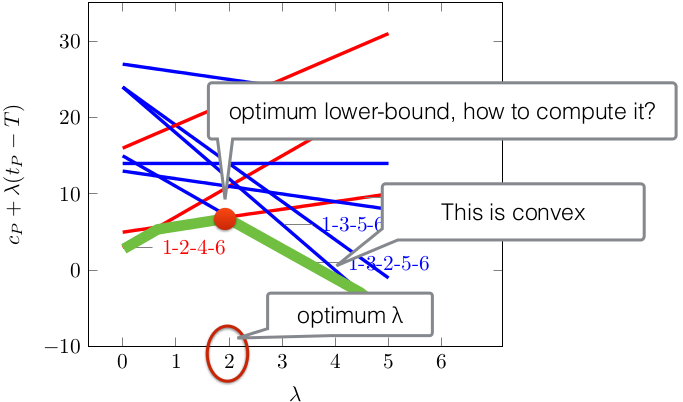
\includegraphics[width=9cm]{lag}
    &
    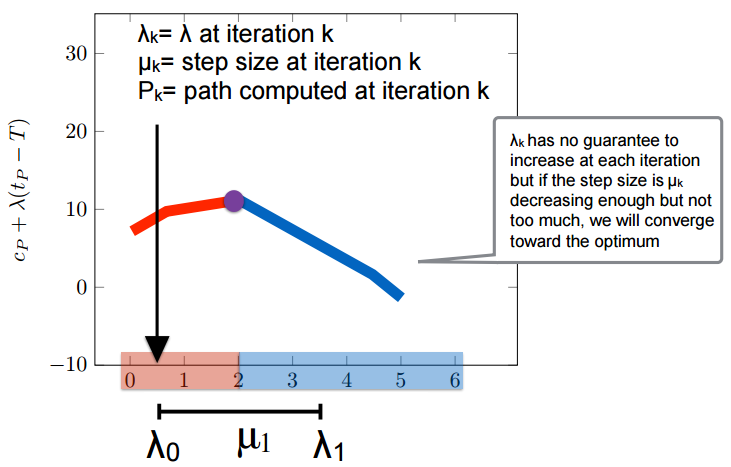
\includegraphics[width=7cm]{lagrangiangraph.png}
\end{tabular}



\paragraph{Computing optimum $\lambda$}
Note that $\lambda_0 = 0$
\begin{enumerate}
    \item At iteration $k$, if $P_k$ violate times constraint increase
        $\lambda$ else decrease it 
        $$\lambda_{k+1} = max(0, \lambda_k + µ_k(t_{P_k} - T))$$

    \item $µ_{k+1} = \frac{1}{k}$
\end{enumerate}

\paragraph{Convergence}

\begin{itemize}
    \item In order for the algorithm to converge we must reduce the size
        of the step at each iteration. 
    \item It is guaranteed to converge if $\mu_{k} \rightarrow 0$ and
        $\sum^{k}_{j=1} \mu_{k} \rightarrow \infty$.
    \item On the other hand the Lagrangian lower bounds has no
        guaranteed to increase at each step.
    \end{itemize}

\paragraph{Pseudo-code}:

\begin{tabular}{m{9cm}m{6cm}}
\begin{lstlisting}[mathescape]
// Result: A lower bound L* and a potentially good (not proven optimal) feasible candidate path P*
L* = $-\infty, \quad k = 0, \quad µ_0=1, \quad \lambda_0 = 0$
P* = shortest path using weights $t_{ij}$
if ($t_{p*} > T$) then
    return 'unfeasible'

while($µ \geq \epsilon$) do
    // Compute shortest path $P_k$ using 
    // weights $c_{ij} + \lambda_k t_{ij}$
    $L_k = c_{P_k} + \lambda_k \bigg(t_{P_k} - T \bigg)$
    if $L_k \geq L*$ then
        $L* = L_k$
        if $P_k$ is feasible then
            $P* = P_k$

    Udate $\lambda_k$ and $µ_k$
    k = k+1
\end{lstlisting}
&
It has not guarantee to find the best
one. But we have a lower-bound at
if P k is feasible then
the end thus we can compute the
« gap »: $$(C_{P_k} - L*)/L*$$
The gap should be non decreasing.
\end{tabular}

\paragraph{Performances}

The Lagrangian relaxation is as good as the linear relaxation. But the
advantage of the Lagrangian one is that it will return feasible solution
during the process.

Typically the lower bounds will evolve along a curve that converge after x steps.

\centerline{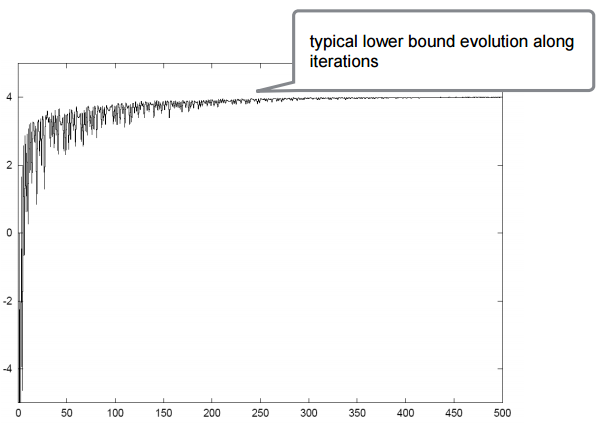
\includegraphics[scale=0.8]{lagrangeconverge.png}}

